\clearpage
\newpage

\chapter{System architecture}
\label{cha:4}

\begin{figure}[t]
  \begin{center}
   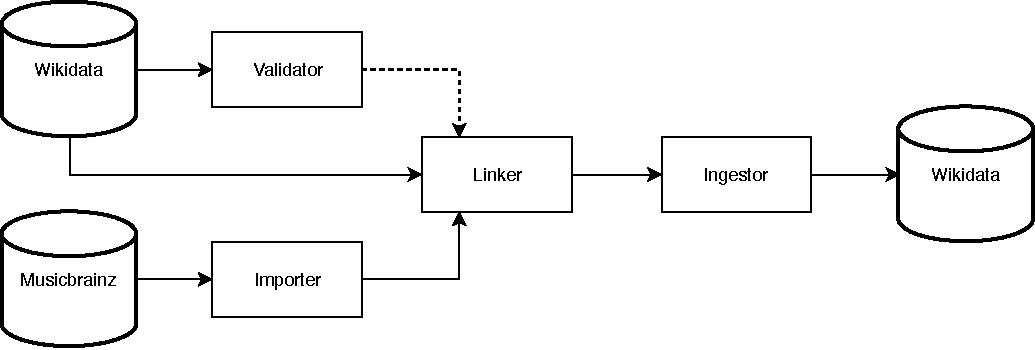
\includegraphics[width=\textwidth]{images/archi2.pdf}
   \captionof{figure}{\texttt{soweego} architecture overview}
   \label{fig:architecture}
  \end{center}
\end{figure}

\texttt{soweego} is a pipeline that performs several tasks in order to link entities between Wikidata and the target database. We drive the description by means of our work on \texttt{MusicBrainz}.\footnote{\url{https://musicbrainz.org}} \texttt{MusicBrainz} is a community-maintained open-source database of music information.\footnote{\url{https://musicbrainz.org/doc/About}} Given our people use case, we focus on the subset of musical artists.

\section{Importer}
\label{cha:41}
The importer module is in charge of downloading the latest target database dump and store it in an internal database table. The importer is designed to slice the dump in order to only keep the desired subset. Since \texttt{soweego} processes different databases, a configurable middleware takes care of the task. The middleware allows to pre-process the data and to map it against our extendable model. The core model is as follows:
\begin{itemize}
    \item \textit{Catalog ID}, i.e., the identifier of the entity in the target database;
    \item \textit{Label}, i.e., the full name;
    \item \textit{Birth Date};
    \item \textit{Birth date precision};
    \item \textit{Death Date};
    \item \textit{Death date precision}.
\end{itemize}
The extendable schema allows to leverage the peculiarities of the targets, while shared procedures can be applied thanks to the core model.

A common issue (in music databases above all) is people having multiple names, known as \textbf{aliases}. The schema easily handles them by treating the aliases as standalone entities. Clearly, these standalone entities duplicate all the original entity data, except the label. Since the pipeline only reads from the database, a de-normalized approach naturally fits better than a normalized one.

The import phase actually attempts to create two tables: one as described above, and one for the \textbf{external links}. External links are valid URLs pointing to additional resources out of the target database. The core model chosen for links is as follows:
\begin{itemize}
    \item \textit{Entity ID}, i.e., a foreign key to retrieve the person information;
    \item \textit{URL}, i.e., the original full link available in the dump;
    \item \textit{Tokens}, i.e., a tokenized version of the link.
\end{itemize}
The \textit{tokens} attribute contains the link without the \textit{meaningless} words of a well-formed URL, such as \texttt{http}. This is inspired by Natural Language Process (NLP) techniques for highlighting the semantics of a text. For instance, the tokenized link does not distinguish the same resource referenced by \texttt{m.facebook.com} or \texttt{facebook.com}.


\section{Linker}
\label{cha:42}
The linker module is the core engine of the whole system: it is in charge of linking Wikidata to the chosen target database. At the time of writing this thesis, it does not exploit any statistical/probabilistic approach, such as neural networks. It is instead implemented as a set of rule-based linking strategies. A machine learning approach will probably be explored in the further steps. The rule-based linking strategies can be viewed as a set of features for a probabilistic classifier.

\subsection{Perfect name match}
\label{cha:421}
Checking if two human entities share the same full name is the most straightforward linking strategy, but it is prone to many errors. First, it fails at homonyms disambiguation; second, it is not tolerant against string differences. For instance, people with a second name like \textit{George Walker Bush} can appear also as \textit{George Bush} or \textit{George W. Bush}. On top of that, the label \textit{George Bush} is ambiguous because it can refer to both \textit{George Bush junior} or \textit{George Bush senior}.
To reduce the amount of ambiguous entities, we apply this strategy to a relevant source database subset. In the case of \texttt{MusicBrainz}, we slice the musicians subset out of Wikidata. As observed in the example above, this heuristic does not completely solve the problem: for instance, both the \textit{Bushes} were politicians.

\subsection{Perfect name with birth and death dates match}
\label{cha:422}
The perfect name match strategy can be improved by involving other attributes in the process. The \textit{George Bush} ambiguity described above is easily solved through the birth date attribute. However, the availability of dates can be an issue. In fact, dates can be missing or with low precision (e.g., month or day may be missing). Therefore, the dates match can only deal with the least precise shared date.
Some math built on the \textit{birthday problem}\footnote{\url{https://en.wikipedia.org/wiki/Birthday_problem}} gives us an idea of how likely is to have homonyms with same full birth date.\footnote{\url{https://www.capgemini.com/2011/09/same-name-same-birth-date-how-likely-is-it/}}
Nevertheless, we expect that our use case databases do not fall into this problem, since they do not cover all existing people.

\subsection{Cross-database URL match}
\label{cha:423}
As widely mentioned in this thesis, multiple Web sources may represent the same entity (humans in our case). In general, there is a one-to-many relationship between an entity and its representations in the Web, such as a Twitter profile, a MusicBrainz page, a Wikidata item, etc.
Indeed, we can consume the low-hanging fruits of such multiple representation at linking time: as a rule of thumb, two database entries can be linked if they share an URL pointing to the same resource. In some optimal cases, MusicBrainz can even contain Wikidata entity URLs.

Wikidata does not explicitly expose external links: it is rather a combination of an \texttt{external ID} and a \texttt{URL formatter}. A valid reference to the external source can be built from these data.

The naïve linking strategy is a perfect string match between computed Wikidata URLs and the target database ones. However, it is not robust to URL heterogeneity: for instance, it fails when one URL starts with \texttt{http} and the other with \texttt{https}. Making a Web request to these two URLs and comparing the response would be the most suitable way to assess their equality. Still, it would bears a significant latency in code execution.

We improve the strategy robusness by taking inspiration from NLP techniques.
The intuition is that there are many variable parts in a valid URL: for instance, \texttt{http} versus \texttt{https}, the presence or absence of a trailing slash \texttt{/}, of leading \texttt{www} or \texttt{m}, and so forth.
Consquently, we tokenized the URL and removed \textit{stop words} like the aforementioned ones. For instance, \url{https://twitter.com/GeorgeHWBush} would become \texttt{['twitter', 'com', 'GeorgeHWBush']}.

\subsection{Normalized full names match}
\label{cha:424}
As described in Section~\ref{cha:422}, the perfect name match strategy has some flaws. For instance, \textit{Vladimir Vladimirovič Putin} or \textit{vladimir vladimirovič putin} would not match, due to the different usage of capital letters. Another issue arises when comparing different language alphabets, such as Latin \textit{Vladimir Vladimirovič Putin} and Cyrillic \begin{otherlanguage}{russian}\textit{Владимир Владимирович Путин}\end{otherlanguage}.
There are many normalization techniques that help reduce the impact of these problems. The first problem is easily solved by always working with lowercased strings; the second one requires transliteration\footnote{\url{https://en.wikipedia.org/wiki/Transliteration}} of non-Latin alphabets into Latin via conventional conversion tables. In addition, diacritics get normalized to the ASCII character set, thus solving mismatches due e.g., to accents omission.
Finally, word tokenization takes place, resulting in a set of tokens from the normalized string. Tokenization is implemented as a string split by non-word characters, specificially through the regular expression \verb@\W+@.

\section{Ingestor}
\label{cha:43}
The main goal of the system is to improve Wikidata content: hence. confident output should be directly added. Wikidata bots\footnote{\url{https://www.wikidata.org/wiki/Wikidata:Bots/}} are non-human users allowed to perform high-volume edits. A bot account must first undergo community discussion for eventual approval, since it can damage a lot of data.
Specifically, \texttt{soweego} adds confident output to Wikidata through a bot included in the ingestor module, while we plan to upload non-confident output to the \texttt{Mix'n'match}\footnote{\url{https://tools.wmflabs.org/mix-n-match/}} tool, which enables human curation of identifier matches.
The first approved task\footnote{\url{https://www.wikidata.org/wiki/Wikidata:Requests_for_permissions/Bot/soweego_bot}} of the \texttt{soweego bot}\footnote{\url{https://www.wikidata.org/wiki/User:Soweego_bot}} is the addition of links in the form of \texttt{External ID}\footnote{\url{https://www.wikidata.org/wiki/Wikidata:Glossary/en\#External_identifier}} \textit{claims},\footnote{\url{https://www.wikidata.org/wiki/Wikidata:Glossary/en\#Claim}} or \textit{references}\footnote{\url{https://www.wikidata.org/wiki/Wikidata:Glossary/en\#Reference}} whenever the claim already exists.


\section{Validator}
\label{cha:44}
Given a target database, the validator module retrieves already linked Wikidata entities and performs validation checks according to a set of criteria. First, dead or wrong identifiers should be removed. More specifically, the target database may not contain the entity anymore or the entity may have moved to another identifier. In these cases, the validator interacts with the ingestor to remove the invalid link.
In the subsequent run, the linker module will also propose matches to those entities that were affected, thus potentially fixing eventual validation errors.

The second validation criterion relies on a set of essential attributes, namely gender, birth date, birth place, death date, and death place. Clearly, a check over this criterion can only run if both the Wikidata and the target database entities share at least a subset of these attributes. In case of mismatches, the link is marked as invalid and the validator sends it to the ingestor for deprecation.

We foresee the implementation of more fine-grained checks focusing on data consistency. For instance, a dead person cannot be married after the death date.
The validator module will play a central role in the final system: first, it will serve as a tool to detect divergence between Wikidata and a target database; second, it will be responsible of the training set construction for linking strategies based on machine learning.

